% Bartosz Bednarczyk
% Analiza numeryczna sprawozdanie 3

\documentclass{article}

\usepackage{polski}
\usepackage[utf8]{inputenc}

\usepackage{fancyhdr} % Required for custom headers
\usepackage{lastpage} % Required to determine the last page for the footer
\usepackage{extramarks} % Required for headers and footers
\usepackage[usenames,dvipsnames]{color} % Required for custom colors
\usepackage{graphicx} % Required to insert images
\usepackage{listings} % Required for insertion of code
\usepackage{courier} % Required for the courier font
\usepackage{lipsum} 
\usepackage{amsfonts}
\usepackage{amsthm}
\usepackage{hyperref}
\usepackage{tikz}
\usepackage{amsmath}
\usepackage{pdfpages}
\usepackage{mathtools}
\usepackage{amsthm}
\usepackage{float}


\DeclarePairedDelimiter\abs{\lvert}{\rvert}
\DeclareUnicodeCharacter{00A0}{ }

\newtheorem{thm}{Twierdzenie}
\newtheorem{remark}{Uwaga}
\newtheorem{lemat}{Lemat}
\newtheorem{wniosek}{Wniosek}
\newtheorem{definicja}{Definicja}
\newtheorem{ciekawostka}{Ciekawostka}
\newtheorem{przyklad}{Przykład}

\newenvironment{rozw}{\paragraph{Rozwiązanie:}}{\hfill}


\usepackage{inconsolata} % very nice fixed-width font included with texlive-full
\usepackage[usenames,dvipsnames]{color} % more flexible names for syntax highlighting colors
\usepackage{listings}

% Margins
\topmargin=-0.45in
\evensidemargin=0in
\oddsidemargin=0in
\textwidth=6.6in
\textheight=9.0in
\headsep=0.25in

\linespread{1.1} % Line spacing

% Set up the header and footer
\pagestyle{fancy}
\lhead{\hmwkAuthorName} % Top left header
\rhead{\firstxmark} % Top right header
\lfoot{\lastxmark} % Bottom left footer
\cfoot{} % Bottom center footer
\rfoot{Page\ \thepage\ of\ \protect\pageref{LastPage}} % Bottom right footer
\renewcommand\headrulewidth{0.4pt} % Size of the header rule
\renewcommand\footrulewidth{0.4pt} % Size of the footer rule

\setlength\parindent{0pt} % Removes all indentation from paragraphs

%----------------------------------------------------------------------------------------
%	NAME AND CLASS SECTION
%----------------------------------------------------------------------------------------

\newcommand{\hmwkTitle}{Pracownia 3} % Assignment title
\newcommand{\hmwkDueDate}{} % Due date
\newcommand{\hmwkClass}{Analiza numeryczna} % Course/class
\newcommand{\hmwkClassTime}{} % Class/lecture time
\newcommand{\hmwkClassInstructor}{} % Teacher/lecturer
\newcommand{\hmwkAuthorName}{Bartosz Bednarczyk - Sprawozdanie z pracowni nr 3 - Zadanie 24} % Your name

%----------------------------------------------------------------------------------------
%	TITLE PAGE
%----------------------------------------------------------------------------------------

\title{Analiza numeryczna (M) - Pracownia 3 - Zadanie P3.9\\
Całkowanie numeryczne przy podanych wartościach w punktach\\}
\date{Styczeń 22, 2015}
\author{Bartosz Bednarczyk}


%----------------------------------------------------------------------------------------

\begin{document}

\maketitle

\tableofcontents

\section{Bardzo nieformalny wstęp}

Pojęcie całkowania jest z pewnością jedną z najbardziej elementarnych operacji matematycznych. Nic dziwnego, że chcielibyśmy umieć liczyć całki szybko i dokładnie. Smutnym faktem jest to, że liczenie całek jest nudne - każdy kto przebrnął przez podstawowy kurs analizy widzi, że nie ma w tym nic cudownego (choć być może jest to tylko moja opinia). W związku z tym chcielibyśmy zostawić tego typu rzeczy komputerowi - bezdusznej maszynie, która na nasze polecenie wykona nawet najokrutniejszy rozkaz. Wielu wybitnych matematyków parających się czarną magią (czyt. obliczeniami numerycznymi) postanowiło jak najbardziej ułatwić pracę naszym maszynom (w końcu maszyna też człowiek), co doprowadziło do szeregu metod i sposobów obliczających całki za pomocą przedziwnych wzorów. W poniższym sprawozdaniu postaram się uchylić rąbka tajemnicy numerycznego całkowania i udowodnić, że tak naprawdę, magia uprawiana przez numeryków nie jest wcale taka czarna. Szczególnie skupie się na przypadku, w którym całkujemy nieznaną funkcję opierając się tylko na zadanych wartościach w punktach, co wydaje się sensowne np. z powodu eksperymentów fizycznych.

\pagebreak

\section{Całkowanie korzystające z interpolacji funkcji}

%%%%%%%%%%%%%%%%%%%%%%%%%%%%%%%%%%%%%%%%%%%%%%%%%%%%%%%%%%%%%%%%%%%%%%%%%%%%%%%%%%%%%%%%%%%%%%%%%%%%%%%%%%%%%%%%%%%%%%%%%%%%%%%%%%%%%%%%%%%%%%%%%%%%%%%%%%%%%%%%%%%%%%%%%

\subsection{Wielomiany interpolacyjne a całkowanie}

\begin{thm}[\textbf{O jednoznaczności wielomianu interpolacyjnego}]
\label{twr:jednoznacznosc_interpolacyjnego}

Dla podanych parami różnych punktów $(x_0, y_0), (x_1, y_1), \ldots (x_n, y_n)$ istnieje dokładnie jeden wielomian $n$-tego stopnia, który przechodzi przez wszystkie podane punkty.	
\end{thm}

\begin{proof}

Wiemy, że taki wielomian $w(x)$ istnieje, gdyż możemy wyrazić go wzorem:

\begin{equation}
w(x) = \sum_{i=0}^n \ y_i \prod_{j=0, \ j \neq i}^n \frac{x-x_j}{x_i-x_j}
\end{equation}

Co gdyby istniały dwa wielomiany $w_1(x) \neq w_2(x)$ spełniające powyższe założenia? Rozpatrzmy wielomian $r(x) = w_1(x) - w_2(x)$. Ponieważ wielomiany $w_1$ oraz $w_2$ mają stopnień co najwyżej $n$ to wielomian $r(x)$ również ma stopnień co najwyżej $n$. Zauważmy, że z faktu iż $w_1(x_i) = y_i$ i $w_2(x_i) = y_i$ wynika, że $r(x_i) = 0$. Ponieważ takich punktów mieliśmy $n+1$ to wielomian $r(x)$ zeruje się w $n+1$ miejscach. Zatem z zasadniczego twierdzenia algebry $r(x) \equiv 0$. Stąd wniosek, że $w_1 = w_2$.
\end{proof}

\begin{definicja}
Niech $f : \mathbb{R} \longmapsto \mathbb{R}$ będzie ustaloną funkcją. Weźmy dowolne punkty $P_0 = (x_0, f(x_0))$,\\ $P_1 = (x_1, f(x_1)), \ldots, P_n = (x_n, f(x_n))$. Korzystając z twierdzenia \ref{twr:jednoznacznosc_interpolacyjnego} otrzymujemy pewien wielomian $w(x)$ przechodzący przez podane punkty. Taki wielomian nazywamy \textbf{wielomianem interpolacyjnym} funkcji $f$.
\end{definicja}

Wróćmy do naszego zadania. Mamy podane wartości pewnej funkcji $f : \mathbb{R} \longmapsto \mathbb{R}$ w punktach tzw. \textbf{węzłach} $$a = t_0 < t_1 < \ldots < t_{n-1} < t_{n} = b.$$

Żeby policzyć przybliżoną wartość całki funkcji $f$ możemy skonstruować wielomian interpolacyjny $w(x)$ interpolujący funkcję $f$ w węzłach $t_i$, a następnie policzyć całkę z tego wielomianu.
Zatem otrzymujemy następujący wzór (który jest szczególnym przypadkiem tzw. \textbf{kwadratur} \footnote{O kwadraturach więcej można przeczytać w \cite{kincaid}.} ) :

\begin{center}
\begin{tikzpicture}
\node [draw={black}, fill=black!10, very thick, rectangle, rounded corners, inner sep=20pt, inner ysep=10pt] (box){%
    \begin{minipage}{.9\textwidth}

$$
\int_{a}^{b} f(x) \ dx \approx \int_{a}^{b} \left( \sum_{i=0}^n f(t_i) \prod_{j=0, \ j \neq i}^n \frac{x-t_j}{t_i-t_j} \right) \ dx = \sum_{i=0}^n f(t_i) \overbrace{\int_{a}^{b} \prod_{j=0, \ j \neq i}^n \frac{x-t_j}{t_i-t_j} \ dx}^{A_i} = \sum_{i=0}^n f(t_i) A_i 
$$
    \end{minipage}
};
\node[fill={black}, text=white, rounded corners, right=10pt] at (box.north west) {Obliczanie przybliżonej całki za pomocą kwadratur};
\end{tikzpicture}
\end{center}

%%%%%%%%%%%%%%%%%%%%%%%%%%%%%%%%%%%%%%%%%%%%%%%%%%%%%%%%%%%%%%%%%%%%%%%%%%%%%%%%%%%%%%%%%%%%%%%%%%%%%%%%%%%%%%%%%%%%%%%%%%%%%%%%%%%%%%%%%%%%%%%%


\subsection{Wielokrotne zastosowanie metody trapezów}

Ponieważ obliczanie całki zawartej w stałej $A_i$ z powyższych wzorów dla dowolnego $n$ może być ciężkie, spróbujmy przybliżać naszą całkę za pomocą kilku mniejszych całek. Załóżmy, że mamy punkty $t_0, t_1, \ldots, t_n$ w których interpolowaliśmy naszą funkcję. Podzielmy te punkty na pary i policzmy całkę zgodnie ze wzorem:

\begin{equation}
	\int_{t_0 = a}^{t_n = b} f(x) \ dx \ = \ \int_{t_0}^{t_1} f(x) \ dx + \int_{t_1}^{t_2} f(x) \ dx + \ldots + \int_{t_{n-1}}^{t_n} f(x) \ dx = \sum_{k=1}^{n} \int_{t_{k-1}}^{t_k} f(x) \ dx
\end{equation}

Interpolując funkcję $f$ wielomianem w każdym z podanych przedziałów dostajemy:

\begin{equation}
\label{eq:zlozony_wzor_trapezow}
	\int_{t_0 = a}^{t_n = b} f(x) \ dx \ = \ \sum_{k=1}^{n} \int_{t_{k-1}}^{t_k} f(x) \ dx \ \approx \ \frac{1}{2} \sum_{k=1}^{n}  \left( t_k - t_{k-1} \right) \cdot \left [ f \left( t_{k-1} \right) + f \left( t_k \right) \right ]
\end{equation}

Otrzymany wzór (\ref{eq:zlozony_wzor_trapezow})  będziemy nazywać \textbf{złożoną metodą trapezów}.

\begin{remark}
\label{rem:zlozonywzorrtrapezowownoodlegle}
Dla $n$ równoodległych węzłów złożony wzór trapezów (oznaczany przez $T_n$) przyjmuje postać:

$$\int_{a}^{b} f(x) \ dx \ \approx \ T_n = \frac{b-a}{2n} \left [ f(a) + f(b) + 2 \sum_{i=1}^{n-1} f \left( a + i \cdot \frac{b-a}{n}  \right) \right ] $$

Powyższy wzór można zobrazować w następujący sposób:
\begin{figure}[h!]
	\centering
	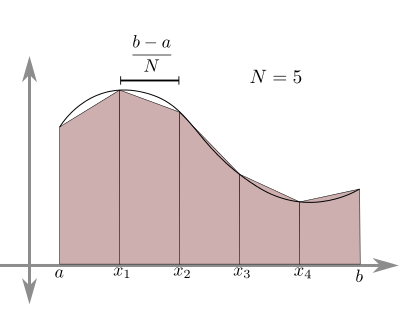
\includegraphics[scale=0.45]{TrapezoidRule}
	\caption{Przybliżanie wykresu funkcji trapezami}
\end{figure}

\end{remark}

\begin{thm}
Jeżeli $f \in C^2$, to błąd złożonego wzoru trapezów wynosi $\frac{-1}{12n^2} (b-a)^3 f''(\xi)$, dla $\xi \in (a,b)$.
\end{thm}

\begin{proof}
Zachęcam do samodzielnego zapoznania się z dowodem dostępnym w artykule \cite{elemprooftrapez}.
\end{proof}

\begin{thm}
\label{thm:trapezy_zbiegaja}
Ciąg złożonych wzorów trapezów z równoodległymi węzłami dla $f \in C^{2}[a,b]$ zbiega do $\int_{a}^{b} f \ dx$.
\end{thm}

\begin{proof}

Z twierdzenia Weierstrassa wiemy, że jeżeli pewna funkcja $g$ jest ciągła na przedziale $[a,b]$ to przyjmuje swoje kresy. Funkcja $f$ podana w zadaniu jest klasy $C^2[a,b]$, czyli  jej druga pochodna jest ciągła na odcinku~$[a,b]$. Stosując twierdzenie Weierstrassa dla funkcji $f''$ otrzymujemy następujące oszacowanie:
$$
\abs*{f - T_n} \ = \ \abs*{\frac{-1}{12n^2} (b-a)^3 f''(\xi_x)} \ \leq \  \frac{h^3}{12n^2} \sup_{x \in [a,b]} f''(x) = C \cdot \frac{1}{n^2}
$$

Ponieważ prawa strona nierówności zbiega do $0$ przy $n \to \infty$, a lewa strona jest nieujemna, to z twierdzenia o trzech ciągach podane wyrażenie również zbiega do $0$, co implikuje tezę zadania.
\end{proof}

%%%%%%%%%%%%%%%%%%%%%%%%%%%%%%%%%%%%%%%%%%%%%%%%%%%%%%%%%%%%%%%%%%%%%%%%%%%%%%%%%%%%%%%%%%%%%%%%%%%%%%%%%%%%%%%%%%%%%%%%%%%%%%%%%%%%%%%%%%%%%%%

\subsection{Wielokrotne zastosowanie metody Simpsona}

Spróbujmy uogólnić metodę z poprzedniego rozdziału. Zamiast przybliżać wykres funkcji trapezami, spróbujmy przybliżać go parabolami. Otrzymany wzór będziemy nazywać \textbf{wzorem Simpsona}.\\

W praktyce sprowadza się to do tego, że podzielmy nasz zbiór węzłów na trójki i dla każdej takiej trójki całkować będziemy interpolujący w nich funkcję $f$ wielomian. Zajmijmy się na razie najprostszym przypadkiem, czyli kiedy nasze węzły $\lbrace t_i \rbrace$ są równoodległe. Łatwo sprawdzić, że :

\begin{figure}[h!]
	\centering
	\includegraphics*[scale=0.55]{simpson_rule}
\end{figure}


\begin{remark}
Dla równoodległych węzłów złożony wzór Simpsona możemy zapisać jako

\begin{equation}
\int_{a}^{b} f(x) \ dx \approx \frac{b-a}{3n} \	\left [ f(t_0) + 4 \sum_{k=1}^{n/2} f(t_{2k-1}) + 2 \sum_{k=1}^{n/2-1} f(t_{2k}) + f(t_{2n}) \right ]
\end{equation}

\end{remark}

Dla lepszego zrozumienia omawianej metody warto zapoznać się z pomocniczym wykresem:

\begin{figure}[h!]
	\centering
	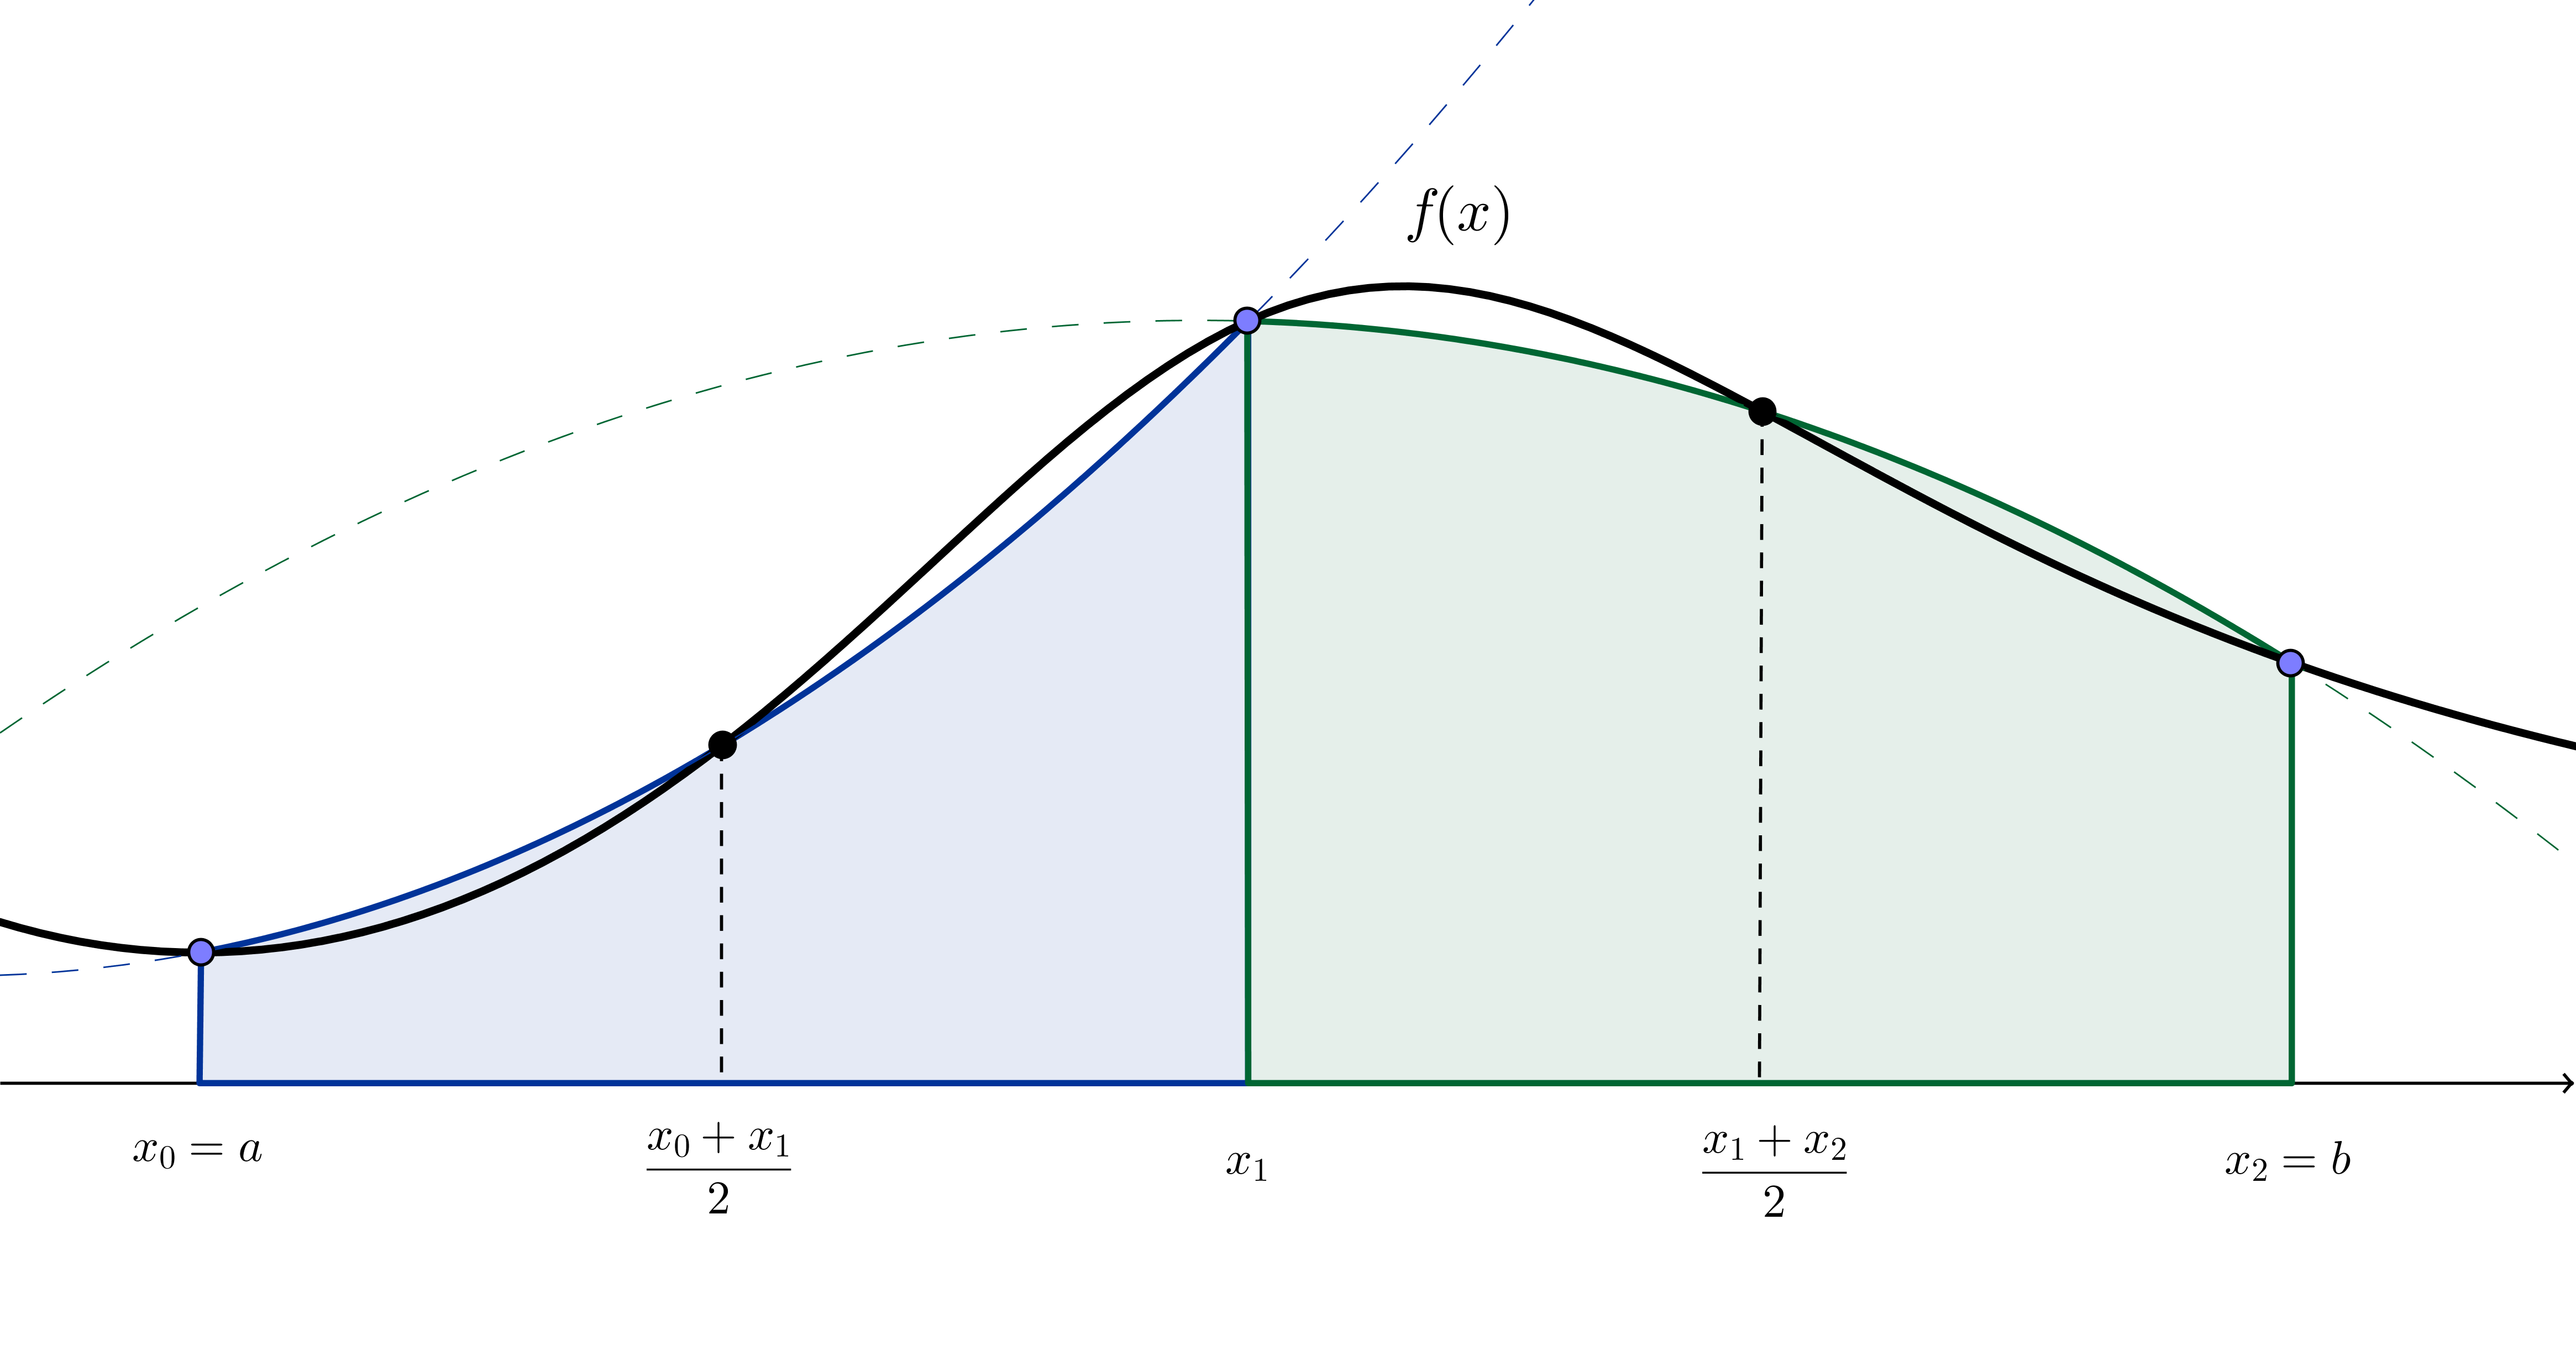
\includegraphics[scale=0.5]{simpson_rule_graph}
\end{figure}

Możemy rozważyć również przypadek, kiedy podane węzły nie są równoodległe. Poniżej przedstawię pełne wyprowadzenie złożonego wzoru Simpsona dla dowolnych parami różnych węzłów $t_i$.


$$\int_{a}^{b} f(x) \ dx \ = \ \sum_{k=1}^{n/2} \int_{t_{2k-2}}^{t_{2k}} f(x) dx \ \approx \ \sum_{k=1}^{n/2} \int_{t_{2k-2}}^{t_{2k}}  \left( \sum_{i=0}^{2} f(t_{2k-2+i}) \prod_{j=0, j \neq i}^{2} \frac{(x-t_{2k-2+j})}{(t_{2k-2+i}-t_{2k-2+j})} \right) = $$

$$
= \sum_{k=1}^{n/2} \int_{t_{2k-2}}^{t_{2k}} \left( \frac{f(t_{2k-2})(x-t_{2k-1})(x-t_{2k})}{(t_{2k-2} - t_{2k-1})(t_{2k-2} - t_{2k})} +  \frac{f(t_{2k-1})(x-t_{2k-2})(x-t_{2k})}{(t_{2k-1} - t_{2k-2})(t_{2k-1} - t_{2k})} + \frac{f(t_{2k})(x-t_{2k-2})(x-t_{2k-1})}{(t_{2k} - t_{2k-2})(t_{2k} - t_{2k-1})} \right) = 
$$

$$
= \frac{1}{6} \sum_{k=1}^{n/2} \left( \frac{f(a)(a-c)(2a-3b+c)}{b-a} + \frac{f(b)(a-c)^3}{(b-a)(b-c)} + \frac{f(c)(a-c)(a-3b+2c)}{b-c}\right), \ \text{gdzie} \ a = t_{2k-2}, b = t_{2k-1}, c = t_{2k}
$$

 
\begin{thm}
Reszta złożonego wzoru Simpsona wynosi $- \frac{1}{2880n^4} (b-a)^5 f^{(4)}(\xi)$, gdzie $\xi \in (a,b)$.	
\end{thm}

\begin{proof}
Analogicznie jak w przypadku wzoru trapezów.
\end{proof}

\begin{thm}
Ciąg złożonych wzorów Simpsona z równoodległymi węzłami dla $f \in C^{4}[a,b]$ zbiega do $\int_{a}^{b} f$.
\end{thm}

\begin{proof}
Analogicznie jak w twierdzeniu \ref{thm:trapezy_zbiegaja} pokazujemy, że reszta zbiega do $0$ przy $n \to \infty$ i korzystamy z twierdzenia Weierstrassa by oszacować czwartą pochodną przez maksimum na podanym przedziale.	
\end{proof}

%%%%%%%%%%%%%%%%%%%%%%%%%%%%%%%%%%%%%%%%%%%%%%%%%%%%%%%%%%%%%%%%%%%%%%%%%%%%%%%%%%%%%%%%%%%%%%%%%%%%%%%%%%%%%%%%%%%%%%%%%%%%%%%%%%%%%%%%%%%%%%%%%%%%%%%%%%%%%%%%%%%%%%%%%%%%

\subsection{Zastosowanie kwadratur o wyższym stopniu}

Rozumowanie przeprowadzone w poprzednich rozdziałach możemy kontynuować zwiększając znowu liczbę węzłów, w których interpolujemy wielomian. Takie podejście ma jednak dużo wad. Po pierwsze zwiększając liczbę węzłów w interpolacji zwiększa nam się stopnień wielomianu interpolacyjnego, co bywa niewygodne w obliczeniach numerycznych. Po drugie całkowanie takiego wielomianu interpolacyjnego jest trudne, o czym można się przekonać patrząc na wyprowadzony przeze mnie złożony wzór trapezów. Trzecią, a zarazem największą wadą, jest możliwość pojawienia się tzw. \textbf{efektu Rungego}.\\

Twierdzenie Stona-Weierstressa mówi, że każdą funkcję ciągłą na przedziale $[a,b]$, o wartościach rzeczywistych, możemy przybliżyć jednostajnie z dowolną dokładnością wielomianami, czyli :

$$
\lim_{n \to \infty} \left(  \max_{a \leq x \leq b} \abs*{f(x) - P_n(x)} \right) = 0.
$$

Jeżeli jednak niewłaściwie dobierzemy węzły, to wraz ze wzrostem liczby węzłów dokładność przybliżenia będzie coraz mniejsza (ciąg powyższych modułów będzie rozbieżny do nieskończoności).

\begin{przyklad}
Rozważmy \textbf{funkcję Rungego} zdefiniowaną jako $f(x) = \frac{1}{1 + 25x^2}$. Będziemy ją interpolować na przedziale $[-1,1]$ wielomianami $P_n$ w równoodległych węzłach postaci $x_i = 2i/n - 1$, dla $i \in \lbrace 0, 1, \ldots, n \rbrace$. Wtedy $\lim_{n \to \infty} \left(  \max_{a \leq x \leq b} \abs*{f(x) - P_n(x)} \right) = \infty$.
\end{przyklad}

\begin{figure}[h!]
\centering
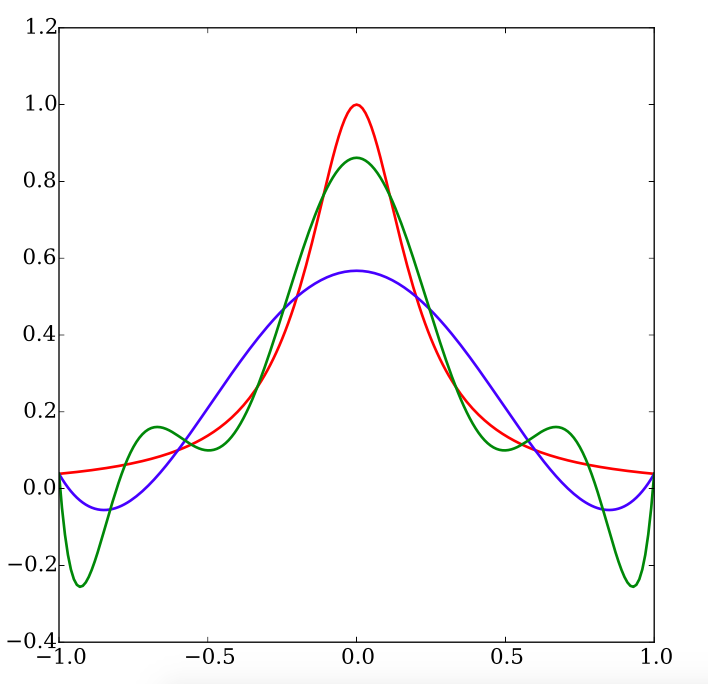
\includegraphics[scale=0.2]{efekt_rungego}
\caption{Czerwony - $f(x)$, zielony - $P_9(x)$, niebieski - $P_5(x)$.}       
\end{figure}

Efekt Rungego bezpośrednio wpływa na wartość obliczanej przez nas całki.\\
Dla przykładu możemy policzyć wartość całki 

$$
\int_{-4}^{4} \frac{dx}{1 + x^2} = 2 \arctan{4} \approx 2.6516353273
$$

przybliżając funkcję wielomianami interpolacyjnymi (w węzłach równoodległych) stopnia $n = 2, 4, 6, 8, 10$.\\
Wyniki obliczeń prezentuję w poniższej tabeli:


\begin{table}[h!]
\centering
\caption{Efekt Rungego dla przykładowej całki}
\label{my-label}
\begin{tabular}{|c|c|c|}
\hline
n  & $\int_{-4}^{+4} P_n(x) \ dx$ & Różnica wyników \\ \hline
2  & 5,49 & 2.83               \\ \hline
4  & 2,27 & 0.38               \\ \hline
6  & 3,32 & 0.66               \\ \hline
8  & 1,94 & 0.71               \\ \hline
10 & 3,59 & 0.93              \\ \hline
\end{tabular}
\end{table}

\begin{wniosek}
Patrząc na tabelę można zauważyć, że rzeczywiście do pewnego momentu wartość całki jest dokładniejsza, po czym stopniowo się pogarsza. Najdokładniejszy wynik jest dla $n = 4$. Nastąpił efekt Rungego. 
\end{wniosek}


%%%%%%%%%%%%%%%%%%%%%%%%%%%%%%%%%%%%%%%%%%%%%%%%%%%%%%%%%%%%%%%%%%%%%%%%%%%%%%%%%%%%%%%%%%%%%%%%%%%%%%%%%%%%%%%%%%%%%%%%%%%%%%%%%%%%%%%%%%%%%%%%%%%%%%%%%%%%%%%%%%%

\pagebreak

\section{Testy numeryczne}

W celu dokładniejszego porównania powyższych wariantów metody obliczania całek wykonane zostały obliczenia komputerowe. Programy zostały napisane w języku Julia 0.4 w środowisku OS X El Capitan i kompilowane za pomocą polecenia \textbf{julia program.jl} w terminalu. Poniżej przedstawiam sześć różnych całek, dla których porównywałem opisane algorytmy.


\subsection{Całkowanie wielomianu $\int_{-1}^{1} 7x^5 + 2x^4 + 3x^3 - 12x - 2 \ dx.$}

\begin{figure}[h!]
\centering
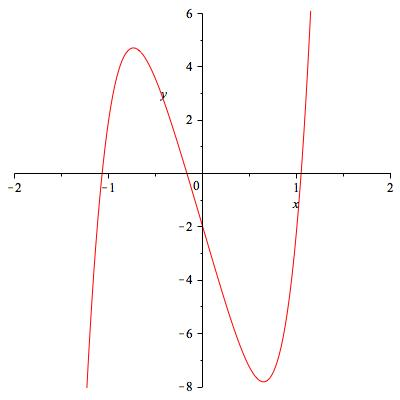
\includegraphics[scale=0.4]{funkcja1_wykres}
\caption{Wykres funkcji $f(x) = 7x^5+2x^4+3x^3-12x-2$.}	
\end{figure}


Zacznijmy od całkowania prostego wielomianu. Poniżej umieszczam wykresy mówiące o tym jak dobre przybliżenia (podane jako liczbę cyfr dokładnych na osi Y, a dokładniej ujemny logarytm z różnicy różnicy wyników) dostajemy przy zmianach liczby węzłów (których liczbę podaję na osi X). Ujemne wyniki oznaczają zaburzenia, na które nie będziemy specjalnie zwracać uwagi.

  \begin{minipage}{\linewidth}
      \centering
      \begin{minipage}{0.35\linewidth}
          \begin{figure}[H]
              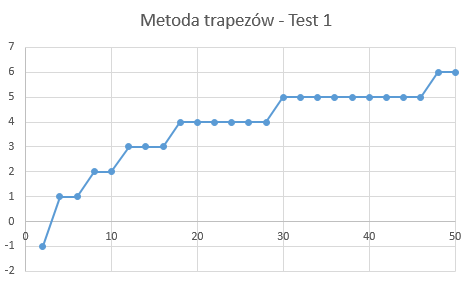
\includegraphics[width=\linewidth]{test_1_trapezy_wykres}
          \end{figure}
      \end{minipage}
      \hspace{0.05\linewidth}
      \begin{minipage}{0.35\linewidth}
          \begin{figure}[H]
              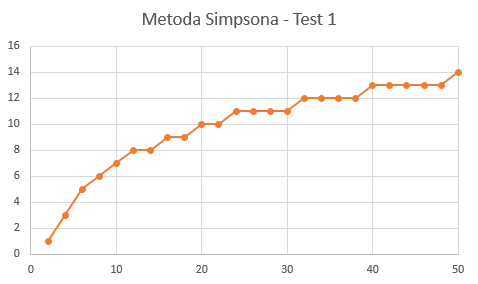
\includegraphics[width=\linewidth]{test_1_simpson_wykres}
          \end{figure}
      \end{minipage}
  \end{minipage}\\

Sprawdźmy jeszcze jak nasze metody zachowują się dla losowych węzłów:

\begin{figure}[h!]
\centering
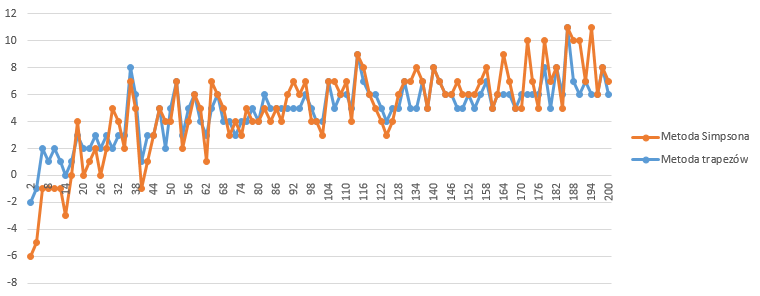
\includegraphics[scale=0.5]{test_1_losowe_wykres}
\end{figure}

\pagebreak

%%%%%%%%%%%%%%%%%%%%%%%%%%%%%%%%%%%%%%%%%%%%%%%%%%%%%%%%%%%%%%%%%%%%%%%%%%%%%%%%%%%%


\subsection{Całka z funkcjami trygonometrycznymi $\int_{-1}^{1} \sin(x^2) - \cos(\sin(x)) + 1 \ dx.$}


\begin{figure}[h!]
\centering
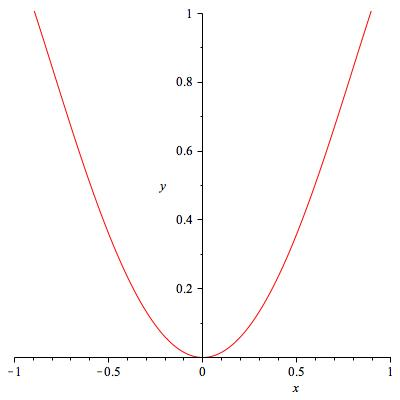
\includegraphics[scale=0.5]{funkcja2_wykres}
\caption{Wykres funkcji $f(x) = \sin(x^2) - \cos(\sin(x)) + 1$.}	
\end{figure}

Popatrzmy jak nasze metody przybliżają złożone funkcje trygonometryczne.


  \begin{minipage}{\linewidth}
      \centering
      \begin{minipage}{0.35\linewidth}
          \begin{figure}[H]
              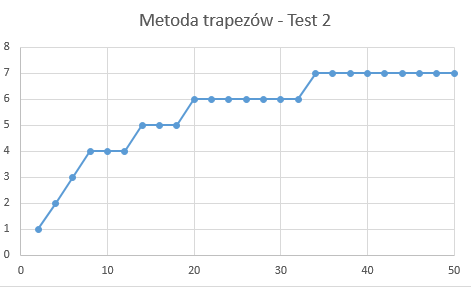
\includegraphics[width=\linewidth]{test_2_trapezy_wykres}
          \end{figure}
      \end{minipage}
      \hspace{0.05\linewidth}
      \begin{minipage}{0.35\linewidth}
          \begin{figure}[H]
              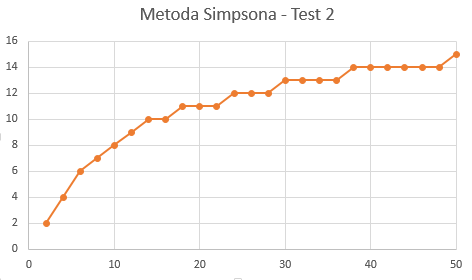
\includegraphics[width=\linewidth]{test_2_simpson_wykres}
          \end{figure}
      \end{minipage}
  \end{minipage}\\


Dla losowych węzłów dostajemy następujące wyniki:

\begin{figure}[h!]
\centering
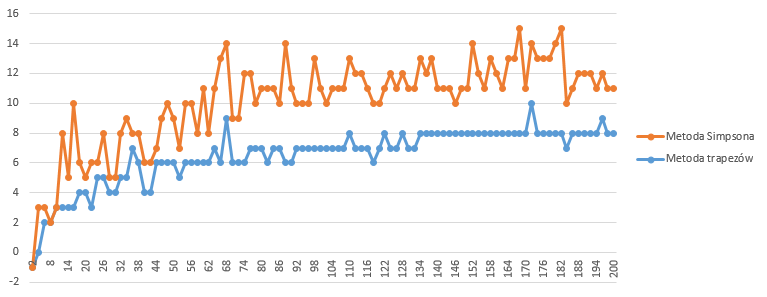
\includegraphics[scale=0.5]{test_2_losowe_wykres}
\end{figure}

W tym i poprzednim przykładzie widać, że złożone wzory Simpsona działają dużo lepiej od wzorów trapezów (zarówno w równoodległych węzłach jak i losowych).
\pagebreak


%%%%%%%%%%%%%%%%%%%%%%%%%%%%%%%%%%%%%%%%%%%%%%%%%%%%%%%%%%%%%%%%%%%%%%%%%%%%%%%%%%%%

\subsection{Całka z funkcji Rungego $\int_{-1}^{1} \frac{1}{1+25x^2} \ dx$ }


\begin{figure}[h!]
\centering
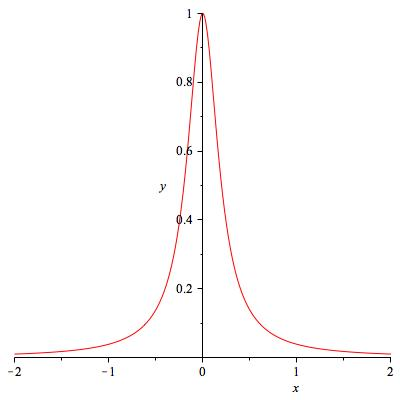
\includegraphics[scale=0.5]{funkcja3_wykres}
\caption{Wykres funkcji Rungego $f(x) = \frac{1}{1+25x^2}$.}	
\end{figure}

Przyjrzyjmy się całkowaniu funkcji Rungego, o której wiemy, że dla kwadratur bywa problematyczna.

  \begin{minipage}{\linewidth}
      \centering
      \begin{minipage}{0.35\linewidth}
          \begin{figure}[H]
              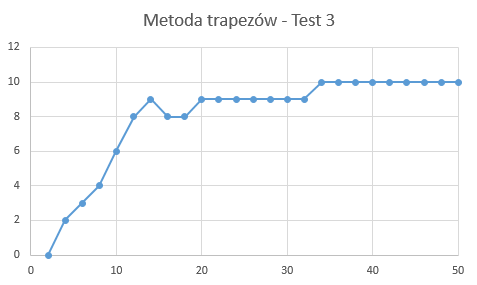
\includegraphics[width=\linewidth]{test_3_trapezy_wykres}
          \end{figure}
      \end{minipage}
      \hspace{0.05\linewidth}
      \begin{minipage}{0.35\linewidth}
          \begin{figure}[H]
              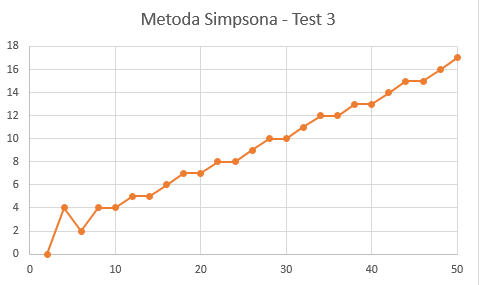
\includegraphics[width=\linewidth]{test_3_simpson_wykres}
          \end{figure}
      \end{minipage}
  \end{minipage}\\


Dla losowych węzłów dostajemy następujące wyniki:

\begin{figure}[h!]
\centering
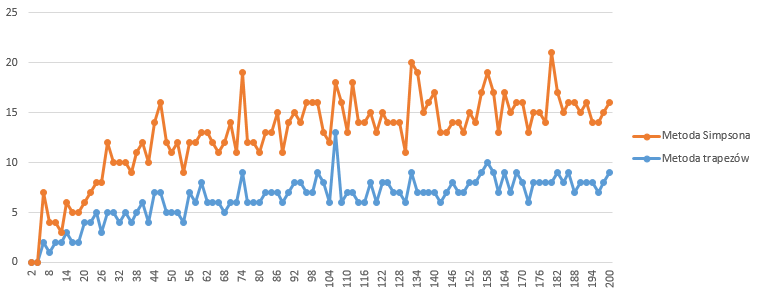
\includegraphics[scale=0.5]{test_3_losowe_wykres}
\end{figure}

Tutaj również obserwujemy wyższość metody Simpsona nad metodą trapezów. Na przykładzie tej funkcji widać, że w pewnym momencie wzór trapezów jest bardzo wolno zbieżny i potrzeba by było naprawdę dużo iteracji by nadgonić wzór Simpsona.

\pagebreak

%%%%%%%%%%%%%%%%%%%%%%%%%%%%%%%%%%%%%%%%%%%%%%%%%%%%%%%%%%%%%%%%%%%%%%%%%%%%%%%%%%%%%%

\subsection{Całka z wielomianu o niskim stopniu $\int_{0}^{10} -x^2 + 5 \ dx $.}


\begin{figure}[h!]
\centering
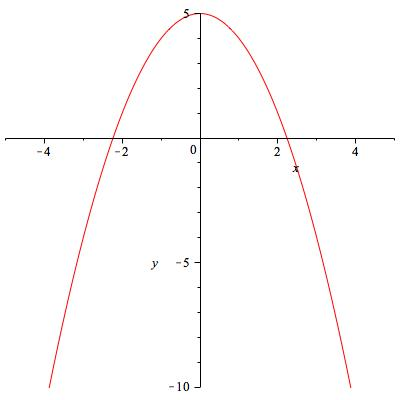
\includegraphics[scale=0.5]{funkcja4_wykres}
\caption{Wykres funkcji $f(x) = -x^2 + 5$.}	
\end{figure}


Nasze kwadratury powinny spokojnie poradzić sobie z czymś tak prostym jak wielomian drugiego stopnia. Spójrzmy na wyniki badań:


  \begin{minipage}{\linewidth}
      \centering
      \begin{minipage}{0.35\linewidth}
          \begin{figure}[H]
              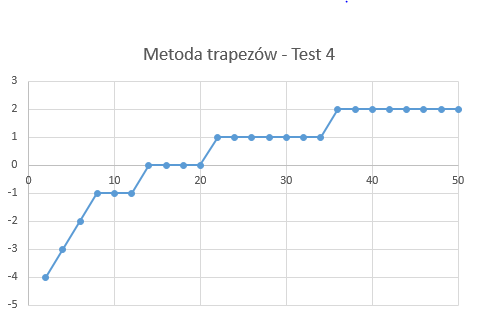
\includegraphics[width=\linewidth]{test_4_trapezy_wykres}
          \end{figure}
      \end{minipage}
      \hspace{0.05\linewidth}
      \begin{minipage}{0.35\linewidth}
          \begin{figure}[H]
              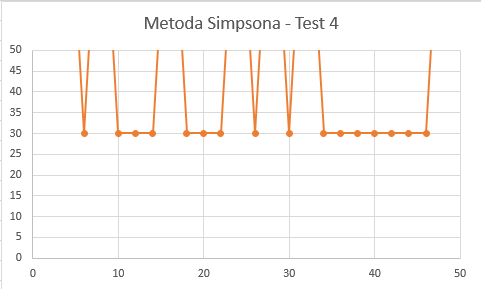
\includegraphics[width=\linewidth]{test_4_simpson_wykres}
          \end{figure}
      \end{minipage}
  \end{minipage}\\

Podczas obliczania wartości całki w losowych węzłach otrzymujemy wynik:

\begin{figure}[h!]
\centering
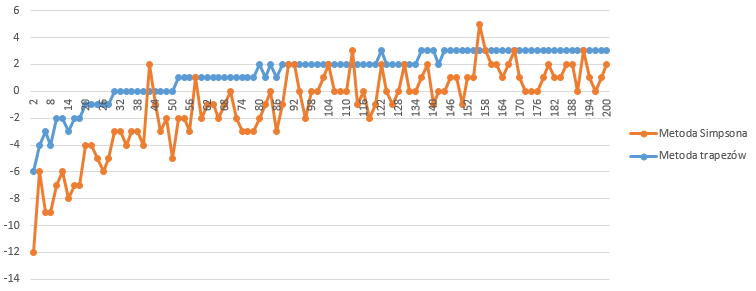
\includegraphics[scale=0.5]{test_4_losowe_wykres}
\end{figure}

Sytuacja jest dość ciekawa. Przy równoodległych węzłach niektóre punkty dla wzoru Simpsona rozbiegają do nieskończoności. Sugeruje to, że dla podanej liczby węzłów dostaliśmy maksymalną dokładność wyniku. Dość zastanawiające jest również to, że dla tej funkcji wzór trapezów działa efektywniej.

\pagebreak

%%%%%%%%%%%%%%%%%%%%%%%%%%%%%%%%%%%%%%%%%%%%%%%%%%%%%%%%%%%%%%%%%%%%%%%%%%%%%%%%%%%%%%


\subsection{Całka z funkcji tworzącej ciągu Fibonacciego $\int_{-1}^{1/2} \frac{1}{1-x-x^2} \ dx$.}

\begin{figure}[h!]
\centering
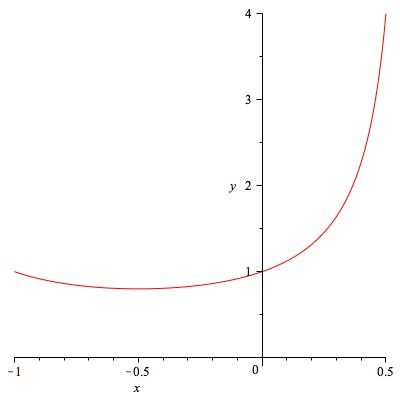
\includegraphics[scale=0.5]{funkcja5_wykres}
\caption{Wykres funkcji tworzącej ciągu Fibonacciego $\int_{-1}^{1/2} \frac{1}{1-x-x^2}$.}	
\end{figure}

Ciekawym przykładem funkcji do zbadania jest funkcja tworząca ciągu Fibonacciego.\\ Wyniki prezentuję poniżej.

  \begin{minipage}{\linewidth}
      \centering
      \begin{minipage}{0.35\linewidth}
          \begin{figure}[H]
              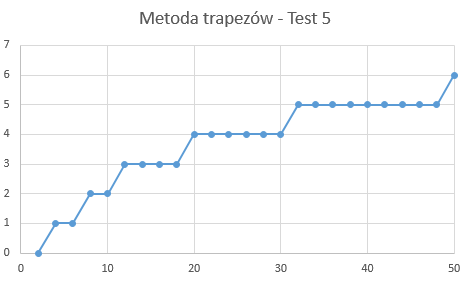
\includegraphics[width=\linewidth]{test_5_trapezy_wykres}
          \end{figure}
      \end{minipage}
      \hspace{0.05\linewidth}
      \begin{minipage}{0.35\linewidth}
          \begin{figure}[H]
              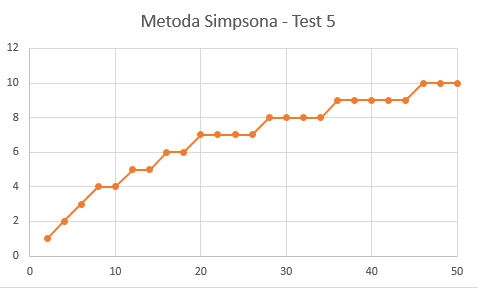
\includegraphics[width=\linewidth]{test_5_simpson_wykres}
          \end{figure}
      \end{minipage}
  \end{minipage}\\

Podczas obliczania wartości całki w losowych węzłach otrzymujemy wynik:

\begin{figure}[h!]
\centering
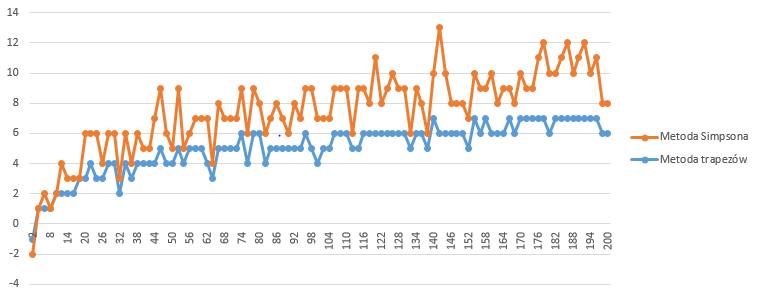
\includegraphics[scale=0.5]{test_5_losowe_wykres}
\end{figure}

Wyniki dla tego przypadku są bardzo podobne jak w pozostałych. Nie wymaga to raczej żadnego komentarza.

\pagebreak

%%%%%%%%%%%%%%%%%%%%%%%%%%%%%%%%%%%%%%%%%%%%%%%%%%%%%%%%%%%%%%%%%%%%%%%%%%%%%%%%%%%%%%


\subsection{Całka z funkcji $\int_{-1}^{1} \exp(x^7) + \cos(2x)+ \arctan(5x) \ dx$.}


Ostatnim prezentowanym przykładem jest całka, która jest sumą najróżniejszych funkcji, które mogłem wymyślić. Podczas konstruowania przykładu starałem się, by kształt wykresu był mocno pofalowany i mało równomierny.


\begin{figure}[h!]
\centering
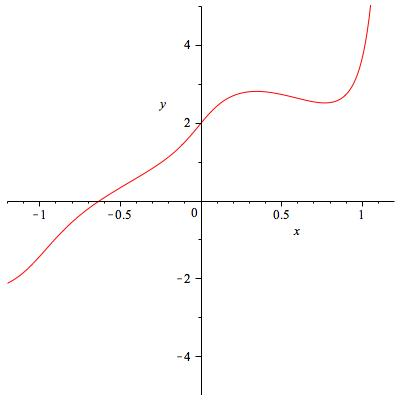
\includegraphics[scale=0.5]{funkcja6_wykres}
\caption{Wykres funkcji $\exp(x^7) + \cos(2x)+ \arctan(5x)$.}	
\end{figure}

  \begin{minipage}{\linewidth}
      \centering
      \begin{minipage}{0.35\linewidth}
          \begin{figure}[H]
              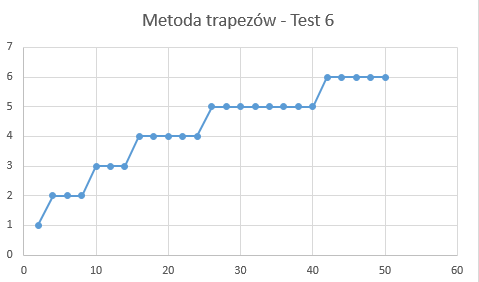
\includegraphics[width=\linewidth]{test_6_trapezy_wykres}
          \end{figure}
      \end{minipage}
      \hspace{0.05\linewidth}
      \begin{minipage}{0.35\linewidth}
          \begin{figure}[H]
              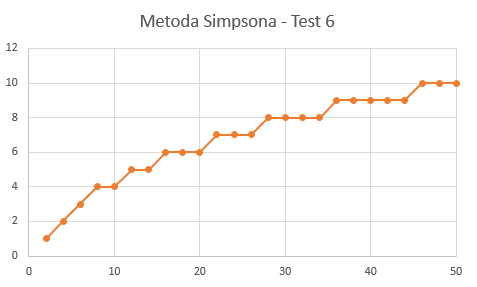
\includegraphics[width=\linewidth]{test_6_simpson_wykres}
          \end{figure}
      \end{minipage}
  \end{minipage}\\

Dokładność całki w losowych punktach dla konkretnych metod możemy zaobserwować na poniższym wykresie. 

\begin{figure}[h!]
\centering
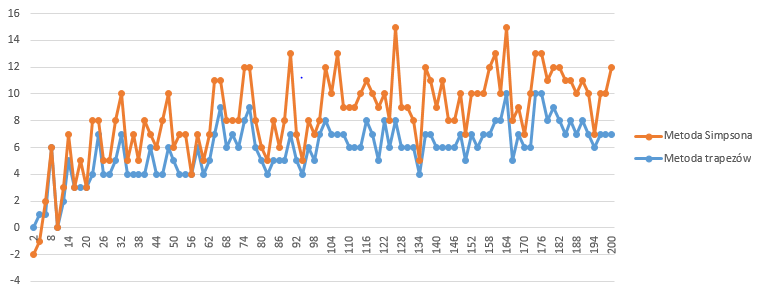
\includegraphics[scale=0.5]{test_6_losowe_wykres}
\end{figure}


%%%%%%%%%%%%%%%%%%%%%%%%%%%%%%%%%%%%%%%%%%%%%%%%%%%%%%%%%%%%%%%%%%%%%%%%%%%%%

\pagebreak

\section{Podsumowanie}

W sprawozdaniu przedstawiłem przykładowe metody obliczania całki w podanych punktach. Zaprezentowałem metodę trapezów i metodę Simpsona, które później złożyłem i otrzymałem tzw. złożone wersje tychże wzorów. Efektywność obu z nich przetestowałem na sześciu przykładach - zarówno w wersji z równoodległymi węzłami jak i losowymi. Pozwolę sobie stwierdzić, że metody nie są jednak zbyt efektywne. Ponieważ nie znamy dokładnie w jakich punktach podane będą wartości funkcji nie możemy skorzystać z ciekawszych kwadratur takich jak np. kwadratury Gaussa, które już przy bardzo niskiej liczbie węzłów całkują o wiele lepiej niż wzór trapezów czy Simpsona. Pozostaje więc niesmak, bo problem dałoby się rozwiązać o wiele dokładniej, gdybyśmy uważniej mierzyli dane. 

\begin{thebibliography}{99}

\bibitem{kincaid} David Kincaid, Ward Cheney, przekł. Stefan Paszkowski,
\emph{Analiza numeryczna},
Warszawa, WNT, 2006.

\bibitem{elemprooftrapez} D. Cruz-Uribe, C. J. Neugebauer,
\emph{An Elementary Proof of Error Estimates
for the Trapezoidal Rule},
Mathematics Magazine, Vol. 76, No. 4 (Oct., 2003), pp. 303-306

\bibitem{SLE} S. Lewanowicz, {\it Analiza Numeryczna - Notatki z wykładu}, Wrocław 2007.

\end{thebibliography}
\end{document}